\documentclass{beamer}
\usepackage[utf8]{inputenc}
\usepackage[spanish]{babel}
\usepackage{hyperref}
\usepackage{verbatim}
\usepackage{listings}
\usepackage{amsmath}

\setbeamercovered{invisible}
\usetheme{Frankfurt}
\usefonttheme{serif}

% Configurar los listings (Códigos)
\renewcommand{\lstlistingname}{Código}
\lstset{
	language=C++,               % Lenguaje
	basicstyle=\ttfamily\tiny,  % Tipo de fuente
	keywordstyle=\color{blue},  % Color de palabras clave
	stringstyle=\color{red},    % Color de strings
	commentstyle=\color{gray},  % Color de comentarios
	showstringspaces=false,     % No muestrar el _ cuando el string tiene espacios
	breaklines = true,          % Partir las líneas largas
	breakatwhitespace=true,	    % Partir las líneas en un espacio
	numbers=left,				% Numerar las líneas a la izq
	numberstyle=\tiny,			% Poner los números de las líneas pequeños
	numberblanklines=true,      % Numerar las líneas en blanco
	columns=fullflexible,       % No perder el formato al dejar los espacios
	keepspaces=true,   			% Dejar los espacios insertados
	frame=tb,					% Poner el recuadro
}

\AtBeginSection[]{%
  \begin{frame}<beamer>
    \frametitle{Contenido}
    \tableofcontents[sectionstyle=show/hide,subsectionstyle=hide/show/hide]
  \end{frame}
  \addtocounter{framenumber}{-1}% If you don't want them to affect the slide number
}

\title{LOOK UP}
\subtitle{Semillero de Programación}
\author{Santiago Vanegas Gil}

\institute{Universidad EAFIT}
\date{30 de agosto del 2014}

\begin{document}

\begin{frame}
	\titlepage
\end{frame}

\begin{frame}
	\frametitle{Contenido}
	\tableofcontents
\end{frame}

\begin{section}{Introducción al Semillero de Programación}
	\begin{subsection}{Descripción}
		\begin{frame}[fragile]
			\frametitle{¿Qué hacemos?}
			Aprendemos varios temas importantes y entrenamos para las maratones de programación de ACIS/REDIS y ACM-ICPC, donde se busca resolver problemas de Ciencias de la Computación conocidos lo más rápido posible.
		\end{frame}
		\begin{frame}[fragile]
			\frametitle{¿Cómo asi?, explícame mejor}
			Podemos ir de lo más simple a lo más complicado:
			\begin{itemize}
				\item Encontrar la cantidad de ocurrencias de una palabra en un texto.
				\item Encontrar la máxima cantidad de basura que puede ser almacenada en un sub-cubo tridimensional, teniendo en cuenta que forma un grafo isomorfo y que el triple de la suma de sus componentes no exceda el producto entre las mismas.
			\end{itemize}
			\pause
			Mentiras, sólo tengan en cuenta que \textbf{casi cualquier problema} puede ser resuelto utilizando programación.
		\end{frame}
		\begin{frame}[fragile]
			\frametitle{¿Dónde es eso?}
			Nos reunimos todos los viernes, de 4 a 6 pm, en el bloque 18, salón 311.
		\end{frame}
	\end{subsection}
	
\end{section}

\begin{frame}[fragile]
	\frametitle{Programas en C++ en consola}
	Para la ejecución de programas por consola
	\begin{itemize}
		\item Escribir el programa.
		\pause
		\item Compilar el programa.
		\pause
		\item Abrir la consola de Windows (Windows + R, escribir cmd).
		\pause
		\item Establecer el directorio en la carpeta del ejecutable del programa.
		\pause
		\item Ejecutar el programa escribiendo el nombre del archivo.
	\end{itemize}
\end{frame}


\begin{section}{Estructuras de datos lineales}

%%  Arreglos  %%
\begin{subsection}{Arreglos estáticos}
	\begin{frame}[fragile]
		\frametitle{Arreglos estáticos}
		\begin{itemize}
			\item{Es una colección de datos secuenciales que son guardados para luego ser consultados basandose en sus índices.}
			\item{Es claramente la estructura más común en maratones de programación.}
			\item{Típicamente se usan arreglos de 1, 2 y 3 dimensiones como máximo.}
			\item{Por ejemplo, un arreglo de 10 posiciones llamado $a$ puede ser representado así:}
			\begin{figure}
				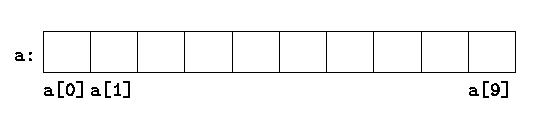
\includegraphics[width = 0.7\textwidth]{src/arreglo.jpg}
			\end{figure}			
		\end{itemize}
	\end{frame}
	
	\begin{frame}[fragile]
		\frametitle{Arreglos estáticos}
		A continuación, aprenderemos cómo declarar arreglos estáticos en C++.
		\begin{block}{Declaración de arreglos estáticos en C++}
			\begin{verbatim}
				tipo_de_dato nombre [número_de_elementos];
			\end{verbatim}
			Ejemplos:\\
			\begin{verbatim}
				int arr [10];
				string words [50];
			\end{verbatim}			
		\end{block}		
	\end{frame}
	
	\begin{frame}[fragile]
		\frametitle{Arreglos estáticos}
		\small{Un ejemplo de uso de arreglos estátios es leerlo y luego recorrerlo hasta encontrar un 0.}
		\begin{lstlisting}
			#include <iostream>
			
			using namespace std;

			const int MAXN = 10;
			int nums[MAXN];
			
			int
			main() {
			    for (int i = 0; i < sizeof(nums) / sizeof(nums[0]); i++) {
			        cin >> nums[i];
			    }
			    for (int i = 0; i < sizeof(nums) / sizeof(nums[0]); i++) {
			        if (nums[i] == 0) {
			            cout << "I found a 0 in position: " << i << endl;
			            break;
			        }
			    }
			    return 0;
			}
		\end{lstlisting}		
	\end{frame}	
\end{subsection}

%%  Vectores  %%
\begin{subsection}{Arreglos dinámicos}
	\begin{frame}[fragile]
		\frametitle{Arreglos dinámicos}
		\begin{itemize}
			\item {Los arreglos dinámicos o vectores son estructuras similares a los arreglos estáticos, excepto que son diseñados para permitir cambio de tamaño en tiempo de ejecución.}
			\item {Al igual que los arreglos, los elementos pueden ser accedidos por medio del índice de su posición, empezando por en índice 0.}
			\item {Las operaciones comúnes en vectores en C++ son: $push\_back()$, operador $[]$ o $at()$, $clear()$, $erase()$, $size()$.}
			\item {En C++, para hacer uso de vectores es necesario importar la biblioteca $vector$, y en Java $ArrayList$.}
		\end{itemize}
		\begin{figure}
			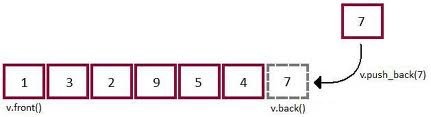
\includegraphics[width = 0.7\textwidth]{src/vector.jpg}
		\end{figure}
	\end{frame}
	
	\begin{frame}[fragile]
		\frametitle{Arreglos dinámicos}
		Veamos un ejemplo del uso de vectores en C++:
		\begin{lstlisting}
			#include <iostream>
			#include <vector> //Remember to include the library

			using namespace std;
			
			int
			main() {
			    vector <int> nums(5, 5); //Initial size 5 with values {5, 5, 5, 5, 5}
			    for (int i = 0; i < nums.size(); i++) {
			        nums[i] = i * 2; //Store new value in position i
			    }
			    for (int i = 0; i < nums.size(); i++) {
			        cout << nums[i] << " ";
			    }
			    //Output will be: 0 2 4 6 8
			    return 0;
			}
		\end{lstlisting}
	\end{frame}

	\begin{frame}[fragile]
		\frametitle{Programa ejemplo 1}
		 Funcionamiento básico de arreglos y vectores
		\texttt{arreglosYVectores.cpp}\\

	\end{frame}
\end{subsection}

%%  Pilas  %%
\begin{subsection}{Pilas}

	\begin{frame}[fragile]
		\frametitle{Pilas}
		\begin{itemize}
			\item {Sólo permite una operación aplicada al tope de la pila, es decir, meter o sacar el último elemento del contenedor.}
			\item {\textbf{El úlltimo elemento que ingresó es el primer elemento en salir (LIFO)}}
		\end{itemize}
		\begin{figure}
			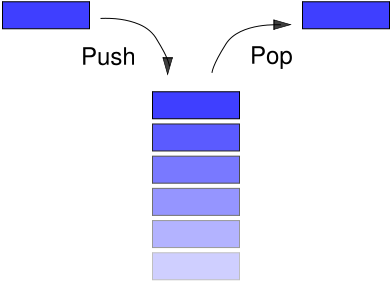
\includegraphics[width = 0.7\textwidth]{src/pila.jpg}
		\end{figure}
	\end{frame}

	\begin{frame}[fragile]
		\frametitle{Pilas}
		Las operaciones que se pueden usar en una pila son:
		\begin{block}{Operaciones soportadas por una pila}
			\textbf{push(x)} - Inserta el elemento x al final de la pila.\\
			\textbf{pop()} - Remueve el último elemento de la pila.\\
			\textbf{top()} - Retorna el último elemento de la pila, sin removerlo.\\
			\textbf{empty()} - Retorna verdadero si la pila está vacía.\\
			\textbf{size()} - Retorna el tamaño de la pila.			
		\end{block}		
	\end{frame}
	
	\begin{frame}[fragile]
		\frametitle{Pilas}
		Veamos un ejemplo de implementación de pila usando la librería de C++ $stack$.
		\begin{lstlisting}
			#include <iostream>
			#include <stack>            // Remember to include stack
			using namespace std;

			int main(){
			   stack <int> s;            // Create an integer stack
			   s.push(10);               // Insert 10
			   s.push(-1);               // Insert -1
			   cout << s.top() << endl;  // Print -1
			   s.pop();                  // Remove -1
			   cout << s.top() << endl;  // Print 10
			   cout << s.size() << endl; // The stack size is 1
			   return 0;
			}
		\end{lstlisting}
	\end{frame}

\end{subsection}


%%  Colas  %%
\begin{subsection}{Colas}
	\begin{frame}[fragile]
		\frametitle{Colas}
		\begin{itemize}
			\item {Las operaciones básicas son insertar al final de la cola, y eliminar del frente de la cola.}
			\item {\textbf{El primer elemento insertado es el primero en salir de la cola (FIFO)}}
		\end{itemize}
		\begin{figure}
			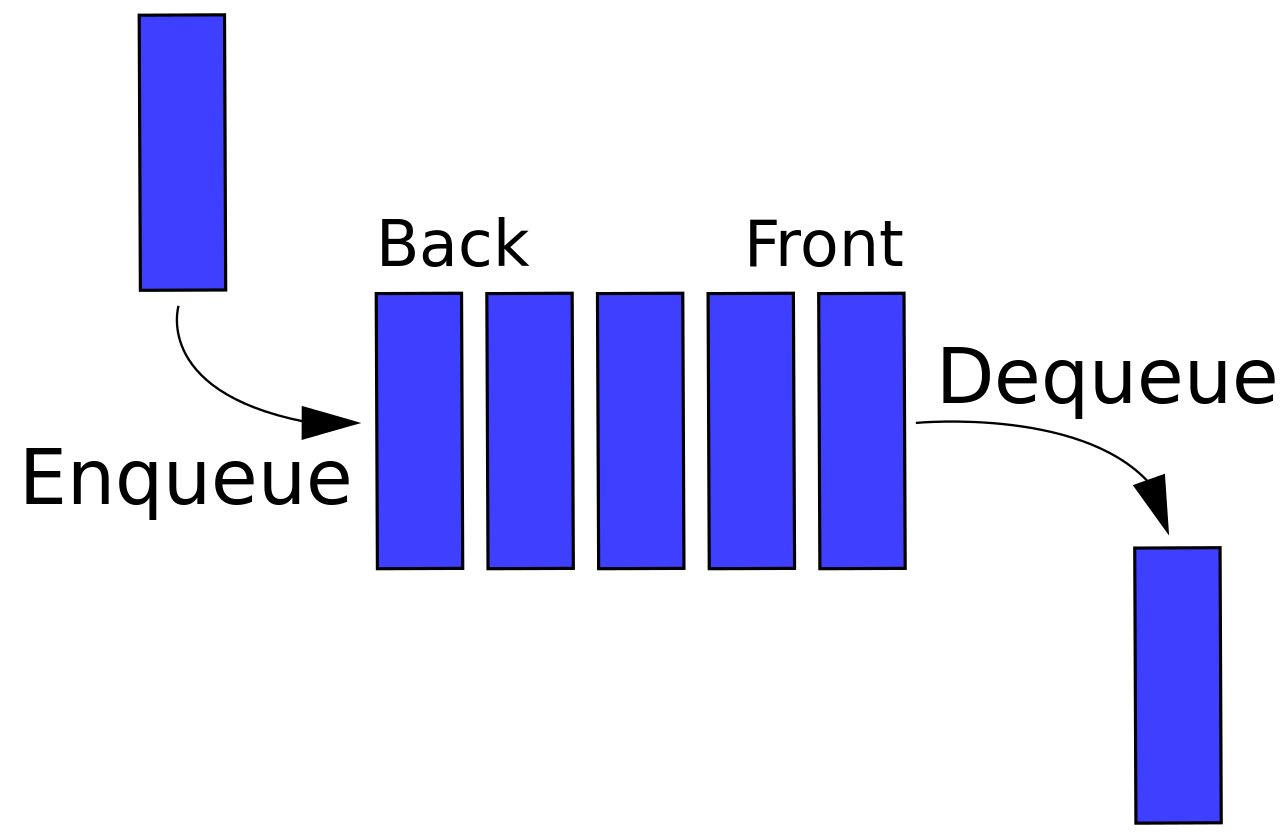
\includegraphics[width = 0.7\textwidth]{src/cola.jpg}
		\end{figure}
	\end{frame}

	\begin{frame}[fragile]
		\frametitle{Colas}
		Las operaciones que se pueden usar en una cola son:
		\begin{block}{Operaciones soportadas por una pila}
			\textbf{push(x)} - Inserta el elemento x al final de la cola.\\
			\textbf{pop()} - Remueve el primer elemento (frontal) de la cola.\\
			\textbf{front()} - Retorna el primer elemento de la cola, sin removerlo.\\
			\textbf{empty()} - Retorna verdadero si la cola está vacía.\\
			\textbf{size()} - Retorna el tamaño de la cola.			
		\end{block}		
	\end{frame}
	
	\begin{frame}[fragile]
		\frametitle{Colas}
		Veamos un ejemplo de implementación de cola usando la librería de C++ $queue$.
		\begin{lstlisting}
			#include <iostream>
			#include <queue>               // Remember to include queue
			using namespace std;

			int main(){
			   queue <int> q;              // Create an integer queue
			   q.push(10);                 // Insert 10
			   q.push(-1);                 // Insert -1
			   cout << q.front() << endl;  // Print 10
			   q.pop();                    // Delete 10
			   cout << q.front() << endl;  // Print -1
			   cout << q.size() << endl;   // The queue size is 1
			   return 0;
			}
		\end{lstlisting}
	\end{frame}

	\begin{frame}[fragile]
		\frametitle{Programa ejemplo 2}
		 Funcionamiento básico de pilas y colas
		\texttt{pilasYColas.cpp}\\

	\end{frame}
\end{subsection}	

\end{section}



\begin{section}{Estructuras de datos no lineales}
	\begin{frame}
		\frametitle{Estructuras de datos no lineales}
		\begin{itemize}
			\item {Para algunos problemas, el almacenamiento lineal no es la mejor opción por su eficiencia en ciertas operaciones.}
			\item {Colecciones dinámicas no lineales como $Maps$ o $Hash Tables$ son las más adecuadas debido a su rendimiento en operaciones de inserción, búsqueda y eliminación.}
		\end{itemize}
	\end{frame}

\begin{subsection}{Arbol binario de búsqueda}
	\begin{frame}
		\frametitle{Arbol binario de búsqueda}
		\begin{itemize}
			\item {Es una forma de organizar los datos en una estructura de árbol.}
			\item {Los items en una rama izquierda de un elemento x son menores que x, y los items en una rama derecha de x son mayores o iguales a x.}
			\item {En C++, implementaciones de árboles binarios de búsqueda están las bibliotecas $map$ y $set$}
		\end{itemize}
		\begin{figure}
			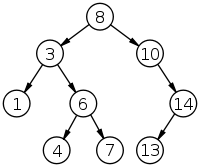
\includegraphics[scale=0.6]{src/bst.jpg}
		\end{figure}
	\end{frame}

%%  Mapa  %%
\begin{subsubsection}{Mapa}
	\begin{frame}[fragile]
		\frametitle{Mapa}
		\begin{block}{Mapa}
			Un mapa es un contenedor que guarda parejas de elementos. El primer elemento de la pareja (key) sirve para identificarla y el segundo elemento (mapped value) es el valor asociado a la llave.\\
		\end{block}
		\begin{block}{Declaración}
			\verb|#include <map>|\\
			\verb|map <tipo_dato_key, tipo_dato_value> nombre;|\\
			Ejemplos:\\
			\verb|map <string, int> m;|\\
			\verb|map <char, int> char2int;|
		\end{block}
	\end{frame}
	
	\begin{frame}[fragile]
		\frametitle{Acceso a elementos de un mapa}
		Los elementos de un mapa se llaman por su llave así:\\ \quad \\
		\verb|map <string, int> m;|\\
		\verb|m["Hola"] = 3;|\\
		\verb|int a = m["Cangrejo"];|\\ \quad \\
		
		Para ingresar un elemento se puede hacer así:\\
		\verb|if (m.count["Nuevo"] == 0) m["Nuevo"] = 123;|\\ \quad \\
		Con la función \verb|count| se busca cuántas veces está el elemento con la llave \verb|"Nuevo"|. Si el elemento no está, cuando accedemos a él con \verb|[]| éste se crea automáticamente.\\
		Cuando accedo con \verb|[]| a un elemento del mapa que no existe este se crea con valores por defecto. Para strings es el string vacío \verb|""| y para enteros es el número 0.
	\end{frame}
	
	\begin{frame}
		\frametitle{Complejidad del mapa}
		\begin{block}{Complejidad}
			\begin{itemize}
				\item Insertar / acceder un elemento al mapa es $O(log\,n \times k)$ donde $n$ es el número de elementos en el mapa y $k$ es el tiempo que toma comparar dos llaves del mapa.
				\item Comparar dos enteros es $O(1)$, comparar dos strings es $O(m)$ donde $m$ es la longitud de los strings.
				\item Insertar / acceder un elemento a un mapa con llaves strings es $O(log\,n \times m)$ donde $n$ son los elementos del mapa y $m$ es la longitud del string.
			\end{itemize}
		\end{block}
		\begin{block}{Nota}
			Los elementos de un mapa se almacenan en orden de acuerdo a una función de comparación. Por defecto la función de comparación es la de menor, es decir que los elementos se almacenan de menor a mayor.
		\end{block}
	\end{frame}
	
	\begin{frame}[fragile]
		\frametitle{Recorrer un mapa}
		Para recorrer un mapa es necesario usar iteradores.\\
		\begin{lstlisting}
		#include <iostream>
		#include <map>
		using namespace std;

		int main(){
		   map <string, int> m;
		   m["b"] = 4;
		   m["bc"] = 1;
		   m["a"] = 3;
		   map <string, int> :: iterator it;
		   for (it = m.begin(); it != m.end(); it++){
		      cout << "( " << it->first << " " << it->second << " ) ";
		      // cout << "( " << (*it).first << " " << (*it).second << " ) ";
		   }
		   return 0;
		}
		// La funcion imprime ( a 3 ) ( b 4 ) ( bc 1 )
		\end{lstlisting}
	\end{frame}
	
	\begin{frame}[fragile]
		\frametitle{Otras funciones en el mapa}
		Otras funciones que se pueden hacer con el mapa son:\\
		\begin{itemize}
			\item Recorrerlo al revés con \verb|rbegin| y \verb|rend|
			\item Obtener el tamaño con \verb|size|
			\item Borrar el contenido con \verb|clear|
			\item Insertar elementos (si no están antes) con \verb|emplace|
			\item Borrar elementos con \verb|erase|
			\item Buscar un elemento con \verb|find|
		\end{itemize}
		\quad \\
		Para más información mirar \url{http://www.cplusplus.com/reference/map/map/}
	\end{frame}
\end{subsubsection}


%%  Sets  %%
\begin{subsubsection}{Set}
	\begin{frame}[fragile]
		\frametitle{Set}
		\begin{block}{Set}
			Un set es un contenedor que guarda conjuntos, es decir grupos de elementos iguales donde cada elemento aparece una sola vez.\\
			Los elementos de un set se almacenan en orden de acuerdo a una función de comparación. Por defecto la función de comparación es la de menor, es decir que los elementos se almacenan de menor a mayor.\\
		\end{block}
		\begin{block}{Declaración}
			\verb|#include <set>|\\
			\verb|set <tipo_dato> nombre;|\\
			Ejemplos:\\
			\verb|set <string> s;|\\
			\verb|set <int> amigos;|
		\end{block}
	\end{frame}

	\begin{frame}[fragile]
		\frametitle{Set}
		Sobre un set se pueden hacer las siguientes operaciones.
		\begin{description}
			\item[insert] Inserta un elemento al set. Ejemplo: \verb|amigos.insert(9)|
			\item[count] Cuenta cuántas veces aparece un elemento (0 o 1 vez). Ejemplo: \verb|amigos.count(3)|
			\item[find] Retorna un iterador al lugar donde está el elemento. Ejemplo: \verb|amigos.find(3)|
			\item[erase] Elimina un elemento del set. Ejemplo: \verb|amigos.erase(amigos.find(3))|
		\end{description}
		Todas las operaciones anteriores tienen una complejidad $O(log\,n \times k)$ donde $n$ es el número de elementos del set y $k$ es el tiempo que toma comparar dos elementos.\\
		Para más información mirar \url{http://www.cplusplus.com/reference/set/set/}
	\end{frame}

	\begin{frame}[fragile]
		\frametitle{Recorrer un set}
		Para recorrer un set es necesario usar iteradores.\\
		\begin{lstlisting}
		#include <iostream>
		#include <set>
		using namespace std;

		int main(){
		   set <int> s;
		   s.insert(4); 
		   s.insert(-1);
		   s.insert(3);
		   s.insert(4);
		   set <int> :: iterator it;
		   for (it = s.begin(); it != s.end(); it++){
		      cout << *it << " ";
		   }
		   return 0;
		}
		// La funcion imprime -1 3 4
		\end{lstlisting}
	\end{frame}
\end{subsubsection}


%%  Colas de prioridad  %%
\begin{subsubsection}{Cola de prioridad}
	\begin{frame}[fragile]
		\frametitle{Cola de prioridad}
		Un heap se puede representar en C++ como una cola de prioridades así:
		\verb|#include <queue>|\\
		\verb|priority_queue <tipo_dato> nombre;|\\
		Ejemplos:\\
		\verb|priority_queue <int> heap;|\\
		\verb|priority_queue <pair <int, int> > q;|\\
		\quad \\
		Para más información mirar: \url{http://www.cplusplus.com/reference/queue/priority_queue/}
	\end{frame}
	
	
	\begin{frame}
		\frametitle{Operaciones}
		La cola de prioridades (heap) soporta las siguientes operaciones
		\begin{description}
			\item [push] Inserta un elemento
			\item [pop] Extrae un elemento
			\item [top] Retorna el máximo elemento de la cola (heap)
			\item [size] Retorna el tamaño de la cola (heap)
		\end{description}
		\quad \\
		La cola de prioridades se ordena de acuerdo a la función de ordenamiento $<$ (menor que) por lo que retorna el elemento con el cual todos los demás comparan menor que él, es decir, el mayor elemento.
	\end{frame}

	\begin{frame}[fragile]
		\frametitle{Para recordar...}
		\begin{itemize}
			\item Ejercicio de entrada y salida de datos por archivo.
			\pause
			\item Ejercicio de leer hasta fin de archivo.
			\pause
			\item Explicación funcionamiento plataforma de juzgamiento BOCA.
			\pause
			\item Asignación de usuarios para comenzar la maratón.
		\end{itemize}
	\end{frame}

	\begin{frame}[fragile]
		\frametitle{Usuarios BOCA}
		\begin{center}
  			\begin{tabular}{| l | l |}
    			\hline
			\textbf{Equipo} & \textbf{Usuario} \\ \hline
   			team1 & Épsilon X \\ \hline
   			team2 & Apocafit \\ \hline
			team3 & decode-team \\ \hline
			team4 & Praise the Sun \\ \hline
			team5 & Los Crafters \\ \hline
			team6 & ENCRYPTED \\ \hline
			team7 & LosSuper op \\ \hline
			team8 & Los PoderOsitos \\ \hline
    			team9 & Pink floyd \\
    			\hline
  			\end{tabular}
		\end{center}
	\end{frame}

	\begin{frame}
		\frametitle{Gracias}
		Esta presentación fue basada en el libro Competitive Programming 3 de Steven Halim y Felix Halim.
		\newline
		Ciertos elementos contenidos en las diapositivas fueron tomados de:\\
		\url{https://github.com/anaechavarria/SemilleroProgramacion/tree/master/Diapositivas}
	\end{frame}
\end{subsubsection}
\end{subsection}
\end{section}
\end{document}